%  LaTeX support: latex@mdpi.com 
%  In case you need support, please attach all files that are necessary for compiling as well as the log file, and specify the details of your LaTeX setup (which operating system and LaTeX version / tools you are using).

% You need to save the "mdpi.cls" and "mdpi.bst" files into the same folder as this template file.

%=================================================================
\documentclass[cryptography,article,submit,moreauthors,pdftex,10pt,a4paper]{mdpi} 
%
%--------------------
% Class Options:
%--------------------
% journal
%----------
% Choose between the following MDPI journals:
% actuators, admsci, aerospace, agriculture, agronomy, algorithms, animals, antibiotics, antibodies, antioxidants, applsci, arts, atmosphere, atoms, axioms, batteries, bdcc, behavsci, beverages, bioengineering, biology, biomedicines, biomimetics, biomolecules, biosensors, brainsci, buildings, carbon, cancers, catalysts, cells, challenges, chemengineering, chemosensors, children, chromatography, climate, coatings, colloids, computation, computers, condensedmatter, cosmetics, cryptography, crystals, data, dentistry, designs, diagnostics, diseases, diversity, econometrics, economies, education, electronics, energies, entropy, environments, epigenomes, fermentation, fibers, fishes, fluids, foods, forests, fractalfract, futureinternet, galaxies, games, gastrointestdisord, gels, genealogy, genes, geosciences, geriatrics, healthcare, horticulturae, humanities, hydrology, informatics, information, infrastructures, inorganics, insects, instruments, ijerph, ijfs, ijms, ijgi, ijtpp, inventions, jcdd, jcm, jcs, jdb, jfb, jfmk, jimaging, jof, jintelligence, jlpea, jmmp, jmse, jpm, jrfm, jsan, land, languages, laws, life, literature, logistics, lubricants, machines, magnetochemistry, make, marinedrugs, materials, mathematics, mca, mti, medsci, medicines, membranes, metabolites, metals, microarrays, micromachines, microorganisms, minerals, molbank, molecules, mps, nanomaterials, ncrna, neonatalscreening, nitrogen, nutrients, ohbm, particles, pathogens, pharmaceuticals, pharmaceutics, pharmacy, philosophies, photonics, plants, polymers, proceedings, processes, proteomes, publications, quaternary, qubs, recycling, religions, remotesensing, resources, risks, robotics, safety, scipharm, sensors, separations, sexes, sinusitis, socsci, societies, soilprocesses, soils, sports, standards, strdrugs, surgeries, sustainability, symmetry, systems, technologies, toxics, toxins, tropicalmed, universe, urbansci, vaccines, vetsci, viruses, vision, water, wem
%---------
% article
%---------
% The default type of manuscript is article, but can be replaced by: 
% addendum, article, benchmark, book, bookreview, briefreport, casereport, changes, comment, commentary, communication, conceptpaper, correction, conferenceproceedings, conferencereport, expressionofconcern, meetingreport, creative, datadescriptor, discussion, editorial, essay, erratum, hypothesis, interestingimages, letter, newbookreceived, opinion, obituary, projectreport, reply, reprint, retraction, review, perspective, preprints, protocol, shortnote, supfile, technicalnote, viewpoint
% supfile = supplementary materials
%----------
% submit
%----------
% The class option "submit" will be changed to "accept" by the Editorial Office when the paper is accepted. This will only make changes to the frontpage (e.g. the logo of the journal will get visible), the headings, and the copyright information. Also, line numbering will be removed. Journal info and pagination for accepted papers will also be assigned by the Editorial Office.
%------------------
% moreauthors
%------------------
% If there is only one author the class option oneauthor should be used. Otherwise use the class option moreauthors.
%---------
% pdftex
%---------
% The option pdftex is for use with pdfLaTeX. If eps figure are used, remove the option pdftex and use LaTeX and dvi2pdf.

%=================================================================
\firstpage{1} 
\makeatletter 
\setcounter{page}{\@firstpage} 
\makeatother 
\articlenumber{x}
\doinum{10.3390/------}
\pubvolume{xx}
\pubyear{2017}
\copyrightyear{2017}
\externaleditor{Academic Editor: name}
\history{Received: date; Accepted: date; Published: date}

%------------------------------------------------------------------
% The following line should be uncommented if the LaTeX file is uploaded to arXiv.org
%\pdfoutput=1

%=================================================================
% Add packages and commands here. The following packages are loaded in our class file: fontenc, calc, indentfirst, fancyhdr, graphicx, lastpage, ifthen, lineno, float, amsmath, setspace, enumitem, mathpazo, booktabs, titlesec, etoolbox, amsthm, hyphenat, natbib, hyperref, footmisc, geometry, caption, url, mdframed, tabto, soul, multirow, microtype, tikz

\usepackage{graphicx}
\usepackage{booktabs}
\usepackage{multirow}
\usepackage{blkarray}
\usepackage{makecell}

%=================================================================
%% Please use the following mathematics environments: Theorem, Lemma, Corollary, Proposition, Characterization, Property, Problem, Example, ExamplesandDefinitions, Hypothesis, Remark, Definition
%% For proofs, please use the proof environment (the amsthm package is loaded by the MDPI class).

%=================================================================
% Full title of the paper (Capitalized)
\Title{A Text-Independent Speaker Authentication System for Mobile Devices}

% If this is an expanded version of a conference paper, please cite it here: enter the full citation of your conference paper, and add $^\dagger$ in the end of the title of this article.
%\conference{Title}

% Author Orchid ID: enter ID or remove command
\orcidauthorONE{0000-0002-0334-6168}
%\orcidauthorTWO{0000-0000-000-000X}
\orcidauthorTHREE{0000-0001-9027-4352}

% Authors, for the paper (add full first names)
\Author{Florentin Thullier $^{1,}$*\orcidONE{}, Bruno Bouchard $^{1}$ and Bob-Antoine J. Ménélas $^{1,}$*\orcidTHREE{}}

% Authors, for metadata in PDF
\AuthorNames{Florentin Thullier, Bruno Bouchard and Bob-Antoine J. Ménélas}

% Affiliations / Addresses (Add [1] after \address if there is only one affiliation.)
\address{%
$^{1}$ \quad Department of Computer Science and Mathematics, Universit\'e du Qu\'ebec \`a Chicoutimi, Chicoutimi, Qu\'ebec, Canada}

% Contact information of the corresponding author
\corres{Correspondence: florentin.thullier1@uqac.ca; bob-antoine-jerry\_menelas@uqac.ca}

% Current address and/or shared authorship
%\firstnote{Current address: Affiliation 3} 
%\secondnote{These authors contributed equally to this work.}
% The commands \thirdnote{} till \eighthnote{} are available for further notes

% Simple summary
%\simplesumm{}

% Abstract (Do not use inserted blank lines, i.e. \\) 
\abstract{This paper presents a text-independent speaker authentication system for mobile devices. A special attention was placed on delivering a fully operational application, which admits a sufficient reliability level, as well as an efficient functioning. To this end, we have excluded the need for any network communication. Hence, we opted for the completion of both the training and the identification processes directly onto the mobile device through the extraction of Linear Prediction Cepstral Coefficients (LPCCs) and the Na\"ive Bayes algorithm as classifier. Furthermore, the authentication decision is enhanced to overcome misidentification through access privileges that the user should attribute to each application beforehand. To evaluate the proposed authentication system, eleven participants were involved in the experiment, conducted in both quiet and noisy environments. Moreover, we also employed public speech corpora to compare this implementation to existing methods. Obtained results have shown that our system is reliable and efficient enough in real use cases. Moreover, we suggest that the proposed authentication system should also be either employed as part of a multilayer authentication, or as a fallback mechanism.}

% Keywords
\keyword{Speaker Authentication; Text-Independent; Mobile Devices; LPCCs; Na\"ive Bayes; Voice; Security}

% The fields PACS, MSC, and JEL may be left empty or commented out if not applicable
%\PACS{J0101}
%\MSC{}
%\JEL{}

%%%%%%%%%%%%%%%%%%%%%%%%%%%%%%%%%%%%%%%%%%
% Only for journal Applied Sciences:
%\featuredapplication{Authors are encouraged to provide a concise description of the specific application or a potential application of the work. This section is not mandatory.}
%%%%%%%%%%%%%%%%%%%%%%%%%%%%%%%%%%%%%%%%%%


%%%%%%%%%%%%%%%%%%%%%%%%%%%%%%%%%%%%%%%%%%
% Only for the journal Data:
%\dataset{DOI number or link to the deposited data set in cases where the data set is published or set to be published separately. If the data set is submitted and will be published as a supplement to this paper in the journal Data, this field will be filled by the editors of the journal. In this case, please make sure to submit the data set as a supplement when entering your manuscript into our manuscript editorial system.}

%\datasetlicense{license under which the data set is made available (CC0, CC-BY, CC-BY-SA, CC-BY-NC, etc.)}

%%%%%%%%%%%%%%%%%%%%%%%%%%%%%%%%%%%%%%%%%%
% For Conference Proceedings Papers:
%\conferencetitle{Add the conference title here}

%\setcounter{secnumdepth}{4}
%%%%%%%%%%%%%%%%%%%%%%%%%%%%%%%%%%%%%%%%%%

\begin{document}
%%%%%%%%%%%%%%%%%%%%%%%%%%%%%%%%%%%%%%%%%%
%% Only for the journal Gels: Please place the Experimental Section after the Conclusions

%%%%%%%%%%%%%%%%%%%%%%%%%%%%%%%%%%%%%%%%%%

\section{Introduction}

Nowadays, mobile devices take a significant place in people\textquoteright s everyday life. As announced by the Gartner Institute, smartphone sales surpassed one billion units in 2014 \cite{1} and people have their mobile devices everywhere and at any time \cite{2} since they are considered as an important part of their life \cite{3}. As a result, users do store private data such as pictures, videos, as well as secret information (\textit{i.e.} emails, bank account) on their devices. However, people are, most of the time, not adequately wary about the safety of these secret information \cite{4}. Within a mobile device context, authentication remains the first entry point for security. Indeed, such a mechanism aims at protecting the digital identity of users.

Over the past few years, various authentication schemes have been proposed. Mobile devices often only offer authentications that involve recalling a piece of information such as PIN code. However, they concede several drawbacks. As an example, it was reported that half of the population do not lock their phone at all \cite{5}. They estimate that entering a PIN code involves lots of inconveniences every time the mobile device has to be unlocked \cite{5}. Moreover, it is known that users have trouble remembering all passwords they use nowadays \cite{6}. It is clear that these behaviors lead a huge impact on the security of mobile devices. Accordingly, people\textquoteright s authentication usages may generate serious threats to the security that a system initially provides \cite{7,8,9}. Recently, biometric authentication mechanisms such as fingerprint, ear shape or gait recognition were enabled on mobile devices \cite{10,11,12,13}. These systems chiefly rely on the uniqueness of the user\textquoteright s physiological or behavioral trait. In the same way, speaker authentication refers to the process of accepting or rejecting a speaker that claims identity. Such schemes are also advised as biometrics since they focus on vocal characteristics produced by the speech and not on the speech only. These features depend on the dimension of the vocal tract, mouth, and nasal cavities, but also rely on voice pitch, speaking style, and language \cite{14}.

Speaker authentication systems may be designed according to two leading methods: text-dependent and text-independent \cite{15,16}. A text-dependent authentication involves the user to pronounce a predefined pass-phrase that is considered as a voice password. It is used both for the enrollment and the identification process. For instance, \textit{Google} recently introduces the trusted voice feature on \textit{Android}, where users have to enroll their voice by pronouncing ''\textit{Ok Google}'' three times. Then, this pass-phrase must be repeated each time the mobile device needs to be accessed. 

By contrast, text-independent schemes are able to identify the user accurately, for any delivered word or locution. Presently, existing speaker authentication techniques offered on mobile devices always require network communications. Indeed, matching templates are usually stored in the cloud. In that sense, they may represent costly authentication solutions for certain users. However, since no additional sensors are needed, they remain inexpensive solutions to authenticate users as regards hardware requirements. Conversely, since manufacturers have pushed fingerprint systems in the forefront of the mobile devices authentication mechanism scene, they tend to become usual. Nevertheless, fingerprints admit a major drawback since they are impossible to use in countries having hard weather conditions as people wear gloves in winter. In that sense, a speaker authentication approach may be a convenient way to resolve such an issue. Moreover, these authentication systems offer a sufficient acceptance rate with end-users and remains less intrusive than fingerprint or retina scan \cite{8,17}. Additionally, these mechanisms may play a major role in some real-world applications to secure identity management systems such as e-commerce solutions, attendance systems, mobile banking or forensics.

It is known that several proposed speaker recognition and identification systems achieve accurate results \cite{18,19,20}. Despite the effectiveness of these mechanisms, few of them are presently implemented on mobile devices. Indeed, they are mostly machine-centered implementations. Moreover, the considerable number of users who still do not secure the access to their mobile devices \cite{5} reveal a need for novel methods mainly focused on a human-centered design that must take into account the diversity of user profiles and usages \cite{21}. This research targets these needs. In that sense, the contribution of this paper is to expose the design of a a text independent speaker authentication system applied to mobile devices that tend to focus on users\textquoteright needs. The choise of a text-independent solution is motivated by a relevant usage when there are social interactions. Indeed, saying ``\textit{Ok Google}'' in the middle of a conversation may be disruptive while a text-independent solution is capable to identify and authenticate the owner of the mobile device all along the conversation without any care for what is being said. Moreover, a recent study \cite{36} highlighted that 62\% of the panel of \textit{Android} users rarely employ the voice assistant feature and most of them have declared that \textit{``they feel uncomfortable talking to their technology, especially in public''}.

The system we propose in this work is a mobile application designed to be extremely convenient for the user. It allows them to forget that they are using a voice-based authentication mechanism. In order to achieve such an authentication, our approach relies on Linear Prediction Cepstral Coefficients (LPCCs) and the Na\"ive Bayes algorithm for patterns classification. Since authentication schemes usually either grant, or deny the access to the whole content of the phone, we further suggest enhancing such a final decision to overcome false positive and negative identification that may occur and reduce annoying situations for the user. Therefore, we introduce the notion of access privileges that enable restricting certain access, based on a simple evaluation of the user\textquoteright s location and the presence of a headset. Moreover, we pay attention to produce an efficient system since we opted for low complexity algorithms and we avoid network communications by achieving both the training and the identification, on the mobile device itself.

The rest of the paper is structured as follows: Section 2 provides an overview of related work to proposed speaker identification and verification systems. Section 3 details the suggested system, specifically designed to entirely operate on mobile devices. Next, section 4 describes experiments we conducted in order to evaluate the reliability as well as the efficiency of such an implementation. Section 5 exposes and discusses results we obtained. Finally, section 6 draws a conclusion and section 7 provides future works.
 
%%%%%%%%%%%%%%%%%%%%%%%%%%%%%%%%%%%%%%%%%%
\section{Related Work}

In order to achieve speaker authentication, several techniques have been described for years through disparate features extraction techniques and classification algorithms. This section first exposes suggested text-independent speaker identification and authentication systems to determine their suitability as regards a usage on mobile devices. Finally, we will examine proposed schemes which were explicitly designed to operate on mobile devices.

First of all, Reynolds and Rose \cite{20} have proposed a text\hyp{}independent speaker identification which exploits Mel-Frequency Cepstral Coefficients (MFCCs) as features and a Gaussian Mixture Model (GMM) to predict which person is speaking. MFCCs are widely used in speaker recognition as they accurately represent the envelope of the short-time power spectrum of the signal. Although such coefficients appear to be more robust against noisy conditions, their acquisition remains very expensive regarding mobile device capabilities \cite{22}. The main motivation of using a GMM was based on an empirical observation that a large number of unlabeled classes of sample distribution, may be represented as a linear combination of Gaussian basis functions. To evaluate the system, a subset of the KING speech database was used. This database provides utterances from speaker conversations over both signal-to-noise radio channels and narrow-band telephone channels. An accuracy of 80.8\% was obtained for 49 telephone speech samples of 15 seconds. Besides, authors claimed that this model is computationally inexpensive and easy to implement on real-time platforms. However, the main drawback of such a system lies in the initialization of the training procedure, where parameters such as mean, covariance and prior of each distribution have to fit the data. Indeed, such a process may be achieved through several costly methods like a Hidden Markov Model (HMM), or a binary k-means clustering algorithm. In that sense, although the identification process may certainly be efficient when used in a mobile device context, the training phase should probably be computationally overly expensive.

Secondly, Kumar \textit{et al.} \cite{18} have suggested another text\hyp{}independent speaker identification approach which aims at predicting utterances thanks to a back-propagation neural network, where LPCs (Linear Prediction Coefficients) parameters were used as input features. The goal of the back-propagation method is to optimize weights between each neuron layers so that, the neural network can learn how to correctly map arbitrary inputs to outputs. Hence, outcomes provide the resulting decision in determining at which speaker corresponds each given utterance. The evaluation of the system was performed over a collection of 25 speech samples in different languages. An overall accuracy measure of 85.74\% was achieved. This led authors to state that such a technique remains appropriate and reliable. However, the theoretical complexity of a standard back-propagation neural network training phase is $O(nmh^k oi)$, where $n$ are training samples, $m$ refers to features, $k$ are hidden layers, each containing $h$ neurons, $o$ refers to output neurons and $i$ is the number of iterations \cite{23}. Hence, such a computation time remains overly expensive in a mobile device context.

On the other hand, concerning speaker authentication, Nair and Salam \cite{19} have proposed a text-independent system which exploits both LPCs and LPCCs to compare their strength. The decision was made through the Dynamic Time Warping (DTW) algorithm. DTW allows calculating the distance between two given sequences which provides the optimal match. Authors have experimented their system over the TIMIT speech corpus which provides 630 real speech signals of American English speakers. An overall accuracy of 92.2\% was obtained with LPCs features while it rose up to 97.3\% with the derivative cepstral coefficients. Combining LPCCs with the DTW algorithm involves thus, an accurate and reliable solution to authenticate users by their voice. Since DTW requires a quadratic time and space complexity (\textit{i.e.} $O(n^2)$) \cite{24}, it may not be the most suitable method to achieve speaker authentication, directly on the mobile device. Nevertheless, real speaker authentication scenarios usually imply few distinct samples. In that sense, DTW as decision-making still stays an acceptable choice for such an authentication mechanism on limited-performance devices.

The growing interest in deep leaning approaches observed in recent years forced to question us about its suitability as regards a speaker identification task. Lee\textit{ et al. }\cite{37} have shown that Convolutional Deep Belief Networks (CDBN) features trained with a SVM classifier have outperformed MFCC features trained with a GMM (respectively to the method described in \cite{38} when the number of training examples was small (\textit{i.e.} 1 to 2 utterances per speaker). However, with a greater number of training samples (\textit{i.e.} 5 to 8 utterances per speaker) results remained similar (\textit{i.e.} around a 99\% accuracy). Moreover, since deep learning algorithms yet remain costly in terms of computational power and processing time, the training process is always achieved on the server-side \cite{39}. However, with the recent partnership developed between \textit{Movidius}, the leader in low-power machine vision for connected devices and \textit{Google}, next generation mobile devices may embed a chip dedicated to the computation of complex machine learning algorithms such as deep neural networks \cite{40}. Then, in the present situation, it appears that such an approach may not be an adequate solution according to our need.

To the best of our knowledge, it appears that few text-independent speaker authentication solutions for mobile devices were applied in practice. For instance, Vuppala \textit{et al.} \cite{25} have suggested a recognition model which lies in several speech enhancements to improve the overall performance faced with different noisy conditions. In that sense, authors aimed to prove the robustness of the method when used in varying background environments. However, their evaluation was performed through noise simulations over speech samples from the TIMIT corpus.

Conversely, Brunet \textit{et al.} \cite{26} have introduced a practical text-independent speaker authentication system which is entirely usable on mobile devices. The approach suggests extracting MFCCs features from speech samples. Then, a reference model is built thanks to a Vector Quantization (VQ) method. The Euclidean distance between stored centroids and testing samples is calculated and compared to a given threshold in order to accept or reject the attempt. Authors have performed an experiment over their own database, where training and testing samples were collected thanks to a mobile device, as well as the Sphinx database which contains 16 American English speakers\textquoteright utterances. Since the method was implemented as a stand-alone biometric system, only the Equal Error Rate (EER) was computed to evaluate the performance. Hence, they obtained better performances on their database (4.52 of EER at best), than the ones on the public database (5.35 of EER at best). However, achieved results largely rely on initial parameters required for the quantization step (\textit{i.e.} the number of centroids) that must be optimized according to the training data. With this brief review, it appears that few text-independent authentications that focus on mobile device computation capabilities and generic usages were proposed. Hence, this paper introduces a user-centered text-independent speaker authentication system for mobile devices. A special attention was paid to its usability and the effectiveness of the training as well as the identification steps in order to compute both of them directly on the mobile device. As a matter of fact, we selected low-computational cost algorithms that do not require any parameter to optimize with others expensive techniques regarding processing time as long as they may offer an accurate identification.

%%%%%%%%%%%%%%%%%%%%%%%%%%%%%%%%%%%%%%%%%%
\section{Proposed Speaker Authentication System}
In this research, we introduce a text independent speaker authentication system for mobile devices. This method works as stand-alone and does not require any costly architectures such as client/server. Hence, the entire computation is done end-to-end on the mobile device. As illustrated in Figure \ref{fig:1}, this mechanism consists of three main processes. The first one involves extracting individual voice features from a raw audio input to build a data set. The following operation lies in training such data with a Na\"ive Bayes classifier. The last process is the authentication decision. It aims at enhancing the conventional speaker verification mechanism to increase the confidence rate of the authentication. To achieve this, we suggest granting a specific access privilege to the user through the evaluation of two different states. The first one concerns the current location of the user that is compared to the ones defined beforehand. Secondly, we evaluate the presence of a headset, that is, whether if it is plugged in the mobile device or not. Indeed, we assume that to use a headset with a built-in microphone reducing surrounding noises will decrease chances for a user to be unwillingly authenticated on this mobile device though replay attacks. \cite{41}

\begin{figure}[H]
	\centering
	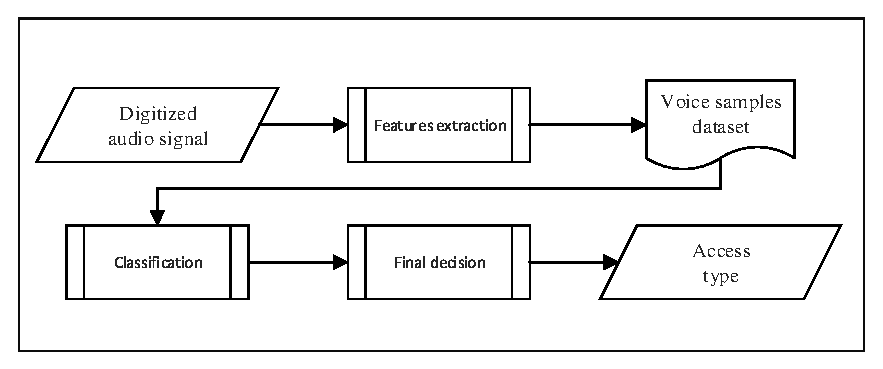
\includegraphics[width=10 cm]{1.eps}
	\caption{Flowchart of our proposed speaker authentication system.}
	\label{fig:1}
\end{figure}

%%%%%%%%%%%%%%%%%%%%%%%%%%%%%%%%%%%%%%%%%%
\subsection{Input}

Audio files are recorded using a 16-bit signed integer PCM encoding format in bi-channels. The sampling rate of such audio files is up to 44.1 kHz.

%%%%%%%%%%%%%%%%%%%%%%%%%%%%%%%%%%%%%%%%%%
\subsection{Pre-processing}

%%%%%%%%%%%%%%%%%%%%%%%%%%%%%%%%%%%%%%%%%%
\subsubsection{Voice Activity Detection (VAD)}

Given an audio record as input, the first step that we produce is a pre-processing phase that aims at removing every silence area only to keep speech segments. To this end, we first have defined a given threshold close to zero (\textit{i.e.} 0.0001). Then, our main focus in such a pre-processing step is to identify which section of the input signal is close to this threshold in order to remove it. To achieve this, we apply the autocorrelation function $r_x (t,k)$ suggested by Sadjadi and Hansen \cite{27} onto a windowed audio segment $s_w (n)$ of the entire input signal $s(n)$ given by, 

\begin{equation}
\label{eq:1}
  r_x(t, x) = \frac{\sum\limits_{n=0}^{N-1}s_w(n)w(n)s_w(n+k)w(n+k)}{\sum\limits_{n=0}^{N-1}					   w(n)w(n+k)}~,
\end{equation}

\noindent where $t$ and $k$ are frame and autocorrelation lag indices, respectively, and $w(n)$ is a Hamming window given by,

\begin{equation}
\label{eq:2}
w(n) = \left\{
		\begin{array}{lll}
			&0.54-0.46 \cos(\frac{2\pi n}{N_w-1}), &0\leq n \leq N_w-1\\
			&0, &otherwise.
		\end{array}\right.~,
\end{equation}

\noindent where its length ($N_w$) is based on the frequency of the signal.

For each processed segment $s_w (n)$, if the mean value of the computed coefficients, resulting from the autocorrelation function, gets close to the defined threshold then, it is identified as a silence area and we finally remove it. Figure \ref{fig:2} graphically illustrates this process.

\begin{figure}[H]
	\centering
	\includegraphics[width=8 cm]{2.png}
	\caption{The first signal is the raw input where silence areas are highlighted. The second is the output of the same signal after the silence removal process.}
	\label{fig:2}
\end{figure}

%%%%%%%%%%%%%%%%%%%%%%%%%%%%%%%%%%%%%%%%%%
\subsubsection{Audio Normalization}

Succeeding the silence removal phase, a peak normalization is performed. The goal is to change the gain of the input to the highest peak of the signal, uniformly. Traditionally, this process is used to ensure that the highest peak remains at 0 dBFS (deciBels relative to Full Scale)\textemdash the loudest level allowed in a digital system. Since the entire signal is adjusted, it is indistinguishable and does not affect the original information. Moreover, the process of normalization ensures that the audio will not clip in any manner. Figure \ref{fig:3} shows the graphical result of such a process.

\begin{figure}[H]
	\centering
	\includegraphics[width=8 cm]{3.png}
	\caption{The left signal is the input signal and the right one is the same signal with peak normalization, where the same sequence is highlighted on both signals.}
	\label{fig:3}
\end{figure}

%%%%%%%%%%%%%%%%%%%%%%%%%%%%%%%%%%%%%%%%%%
\subsection{Feature Extraction}

Since the voice is considered as a signal containing a lot of information about the speaker\textemdash the process of extracting several discriminating features from the speech remains a critical part of both speaker identification and authentication systems. In that sense, we decide to favor the use of the Linear Prediction Cepstral Coefficients (LPCCs). Such coefficients are directly derived from the Linear Prediction analysis that aims at estimating the relevant features or characteristics from a speech signal \cite{28}. We justify such a choice by its ability to provide extremely accurate estimates of the speech parameters, and by its relative speed of computation \cite{22}. This last point was a crucial criterion since mobile devices presently remain less powerful than traditional desktop computers. Figure \ref{fig:4} graphically summarizes the steps of the features extraction from a pre-processed signal to the resulting data set containing voice features.

\begin{figure}[H]
	\centering
	\includegraphics[width=10 cm]{4.eps}
	\caption{Flowchart of the features extraction process.}
	\label{fig:4}
\end{figure}

To compute the LP analysis, we have implemented the Linear Predictive Coding algorithm. It was designed to exploit the redundancy present in the speech signal by assuming that each sample may be approximated by a linear sum of the past speech samples $(p)$. Hence, the predicted sample $S_p (n)$ may be represented as,

\begin{equation}
\label{eq:3}
  S_p(n) = \sum\limits_{k=1}^{p}a_ks(n-k)~,
\end{equation}

\noindent where $a(k)$ are the Linear Prediction Coefficients (LPCs), $s(n-k)$ are past outputs and $p$ is the prediction order. In our case, the speech signal is multiplied by an overlapped Hamming window of 25ms to get a windowed speech segment $S_w (n)$ as,

\begin{equation}
\label{eq:4}
  s_w(n) = w(n)s(n)~,
\end{equation}

\noindent where $w(n)$ is the windowing sequence given in equation (\ref{eq:2}). The error between the actual sample and the predicted one $e(n)$ may be expressed as,

\begin{equation}
\label{eq:5}
  e(n) = s_w(n)-\sum\limits_{k=1}^{p}a_ks_w(n-k)~.
\end{equation}

The main objective of the LP analysis is to compute the LP Coefficients that minimize this prediction error. To this end, our system exploits the autocorrelation method that is usually preferred since it is computationally more efficient and more stable than the covariance one \cite{29}. Thus, the total prediction error $E$ is given as,

\begin{equation}
\label{eq:6}
	E = \sum\limits_{n=-\infty}^{\infty}e^2(n)=\sum\limits_{n=-\infty}^{\infty} 								\left(s_w(n)-\sum\limits_{k=1}^{p}a_ks_w(n-k)\right) ^2~.
\end{equation}

The values of $a(k)$ that minimize this total prediction error may be computed by finding,

\begin{equation}
\label{eq:7}
  	\frac{\delta E}{\delta a_k} = 0,\quad 1\leq k \leq p~.
\end{equation}

Thus, each $a_k$ gives $p$ equations with $p$ unknown variables. The equation (\ref{eq:8}) offers the solution to find LP Coefficients,

\begin{equation}
\label{eq:8}
	\sum\limits_{n=-\infty}^{\infty}s_w(n-i)s_w(n)=\sum\limits_{k=1}^{p}a(k)\sum\limits_{n=-\infty}^{\infty}s_w(n-i)s_w(n-k),\quad 1\leq i \leq p~.
\end{equation}

Consequently, it is possible to express the linear equation (\ref{eq:8}) in terms of the autocorrelation function $R(i)$ as follows,

\begin{equation}
\label{eq:9}
  	R(i) = \sum\limits_{n=i}^{N_w}s_w(n)s_w(n-i),\quad 0\leq i \leq p~,
\end{equation}

\noindent where $N_w$ is the length of the window. Then, by substituting values from equation (\ref{eq:9}) in the equation (\ref{eq:8}) with the autocorrelation function $R(i) = R(-i)$ we obtain the following equation,

\begin{equation}
\label{eq:10}
  	\sum\limits_{k=1}^{p}R(\vert i-k \vert )a_k = R(i),\quad 1\leq i \leq p~.
\end{equation}

The set of linear equations is expressed by the relation $Ra = r$ and may be represented in a matrix form as,

\begin{equation}
\label{eq:11}
	\begin{blockarray}{cccc}
			~ & R & ~ & ~ \\
			\begin{block}{[cccc]}
				R(0) & R(1) & \cdots & R(p-1) \\
				R(1) & R(0) & \cdots & R(p-2) \\
				\vdots & \vdots & \ddots & \vdots \\
				R(p-1) & R(p-2) & \cdots & R(0) \\
			\end{block}
		\end{blockarray}
		\begin{blockarray}{c}
			a\\
			\begin{block}{[c]}
				a_1\\
				a_2\\
				\vdots\\
				a_p\\
			\end{block}
		\end{blockarray}
		=
		\begin{blockarray}{c}
			r\\
			\begin{block}{[c]}
				R(1)\\
				R(2)\\
				\vdots\\
				R(p)\\
			\end{block}
		\end{blockarray}~,
\end{equation}

\noindent where $a$ is the vector of LP coefficients and $r$ is the autocorrelation. The resulting matrix is a Toeplitz matrix where all elements along a given diagonal are equals.

Towards the computation of the LP Coefficient $a_k$, it is possible to derive cepstral coefficients $c_n$ directly through the following relationship,

\begin{equation}
\label{eq:12}
  	c_n = \sum\limits_{k=1}^{n-1}a_k c_{n-k} + a_n,\quad 1<n \leq p~,
\end{equation}

\noindent where $p$ refers to the prediction order.

It is known that speaker recognition requires more cepstral coefficients than speech recognition which employs around 15 of them. Although it was pointed out that increasing the number of such coefficients does not affect the recognition \cite{30}, we suggest using 20 LPCCs to preserve a relatively good computation speed.

%%%%%%%%%%%%%%%%%%%%%%%%%%%%%%%%%%%%%%%%%%
\subsection{Classification}

Several classification algorithms were employed for speaker recognition (\textit{i.e.} GMM, ANN, \textit{etc.}). However, it is known that the Na\"ive Bayes classifier is fast, very effective and easy to implement. As a supervised and statistical learning method for classification\textemdash it simply computes the conditional probabilities of the different classes given the value of attributes. Finally, it selects the class with the highest conditional probability. Accordingly, Table \ref{tab:1} exposes the theoretical time and space complexity evaluations of the Na\"ive Bayes classifier \cite{31}.

\begin{table}[H]
\caption{Naïve Bayes time and space complexities, given $k$ features for both training and testing operations \cite{31}.}
\centering
\label{tab:1}
\begin{tabular}{rcc}
	\hline\noalign{\smallskip}
	\textbf{Operation} & \textbf{Time} & \textbf{Space}  \\
	\noalign{\smallskip}\hline\noalign{\smallskip}\hline\noalign{\smallskip}
		Training on $n$ samples & $O(nk)$ & $O(k)$ \\
		Testing on $m$ samples & $O(mk)$ & $\Theta(1)$ \\
	\noalign{\smallskip}\hline
\end{tabular}
\end{table}

Once the feature extraction process is completed, a set of samples denoted $s_1,s_2,\ldots,s_i$ with their associated class labels $c_{s_1}, c_{s_2}, \ldots, c_{s_i}$, where $c_{s_i}\in \Omega = \{c_1, c_2, \ldots, c_i\}$ is obtained. Each sample has $k$ features (\textit{i.e.} LPCCs) represented by floating numbers (with $k=20$), that are denoted as $a_1,a_2,\ldots,a_n$. The objective of the Na\"ive Bayes classifier is to exploit these samples to build a model (\textit{i.e.} the training phase) that will be reused to predict the label of the class $c_p$ for any future sample (\textit{i.e.} the identification phase). Figure \ref{fig:5} shows a simplified block diagram of this process.

\begin{figure}[H]
	\centering
	\includegraphics[width=10 cm]{5.eps}
	\caption{Flowchart of the classification process.}
	\label{fig:5}
\end{figure}

The algorithm, strongly relies on the Bayes theorem and imposes two assumptions. Firstly, all features $a_1,\ldots,a_n$ should be independent for a given class $c$. This is the class-conditional independence. Secondly, all features $a_1,\ldots,a_n$ should be directly dependent on their assigned class $c$. Given that, it is possible to describe the classifier as,

\begin{equation}
\label{eq:13}
  	P(c\vert a_1, a_2, \ldots , a_n) = \frac{P(c)\prod\limits_{i=1}^{n}P(a_i\vert c)}{P(a_1, a_2, \ldots , a_n)}~.
\end{equation}

Since $P(a_1,a_2,\ldots,a_n )$ is common for a certain sample, it may be ignored in the classification process. As a result, we can derive equation (\ref{eq:13}) to predict the class $c$ of a given sample during the identification phase as follows,

\begin{equation}
\label{eq:14}
  	c = arg~\max\limits_{c\in \Omega } P(c)\prod\limits_{i=1}^{n}P(a_i\vert c)~.
\end{equation}

However, as we obtain the LP coefficients through an autocorrelation method, resulting LPCCs remain strongly dependent and consequently, violate the independence assumption of the Na\"ive Bayes classifier. Nevertheless, Zhang \cite{32} has demonstrated that such a condition is not necessary to satisfy in practical situations. Indeed, no matter how strong dependencies among attributes are, Na\"ive Bayes can still be optimal if they are distributed evenly in class, or if they cancel each other out. Moreover, we have observed that the distribution of our features, for all classes, when compared to their frequency, follows a normal distribution. Hence, it is possible to assume a valuable classification rate with Na\"ive Bayes according to the supposed quality of the LPCCs.

%%%%%%%%%%%%%%%%%%%%%%%%%%%%%%%%%%%%%%%%%%
\subsection{Decision-making}

The result provided by the classification task may return two kinds of errors. On the one hand, a false-negative outcome refers to a failure in a genuine authentication, while a false-positive result concerns an impostor attempt mistakenly identified. According to authentication on mobile devices, false-negative does not compromise the security of the private content. However, it may be disturbing for the user since either the process has to be repeated, or a fallback mechanism has to be used. In contrast, false-positive exhibits a serious vulnerability for the security of such devices since the objective is to avoid fraudulent accesses. Besides, speaker authentication systems are not devoid of other drawbacks that may also lead to security threats. Indeed, they remain vulnerable to voice mimicry or mock authentication through legitimate voice records.

Hence, we suggest improving the authentication process by introducing the notion of access privileges in order to ward against misidentification. The implementation suggested in this paper remains experimental, but it is easily possible to imagine that such a process may become a standard of mobile operating systems. Firstly, we assume that users have assigned a right for each application installed on their mobile device beforehand. Therefore, we define three privileges as follows. The public privilege allows the access to only non-critical content and applications. The protected privilege restricts the access to the most critical pieces of data (\textit{i.e.} bank account). Finally, the private privilege gives the access to the entire content of the mobile device.

The process of determining the safest authority to grant that we suggest begins by verifying the result produced by the identification process. If the voice does not match with a genuine one then, the system allows the user to have a public access. In case of false-negative, the user has to repeat the entire process otherwise, an impostor identification is avoided. If a match does exist, a protected access is granted and the current location is fetched. In that case, the system verifies that the position is inside a given radius between 200 and 500 meters of one trusted location\textemdash where trusted locations refer to a predefined set of places connected with the user (\textit{i.e.} home, work). This verification allows us to be quite more robust against fraudulent authentication attempts. However, a risk still exists, especially when we are facing users living together such as a family or roommates who obviously share at least, one same location. Hence, to reduce chances for a user to be unwillingly authenticated on his own device, we offer to proceed another verification. Indeed, we suggest that the private access level must only be allowed when the authentication process is achieved while using a headset and all previous verification are satisfied. Therefore, we both verify that the headset is plugged into the output of the device and that it provides an extra microphone. We justify such a need because these microphones are closer to the mouth of the speaker and they better filter the surrounding noise than the built-in microphone of the mobile device. Thus, by bypassing the mobile device microphone, we estimate that it represents an additional level of security when there are shared trusted location. In that sense, we assume that false acceptance rates must considerably decrease. Figure \ref{fig:6} graphically summarize this process.

\begin{figure}[H]
	\centering
	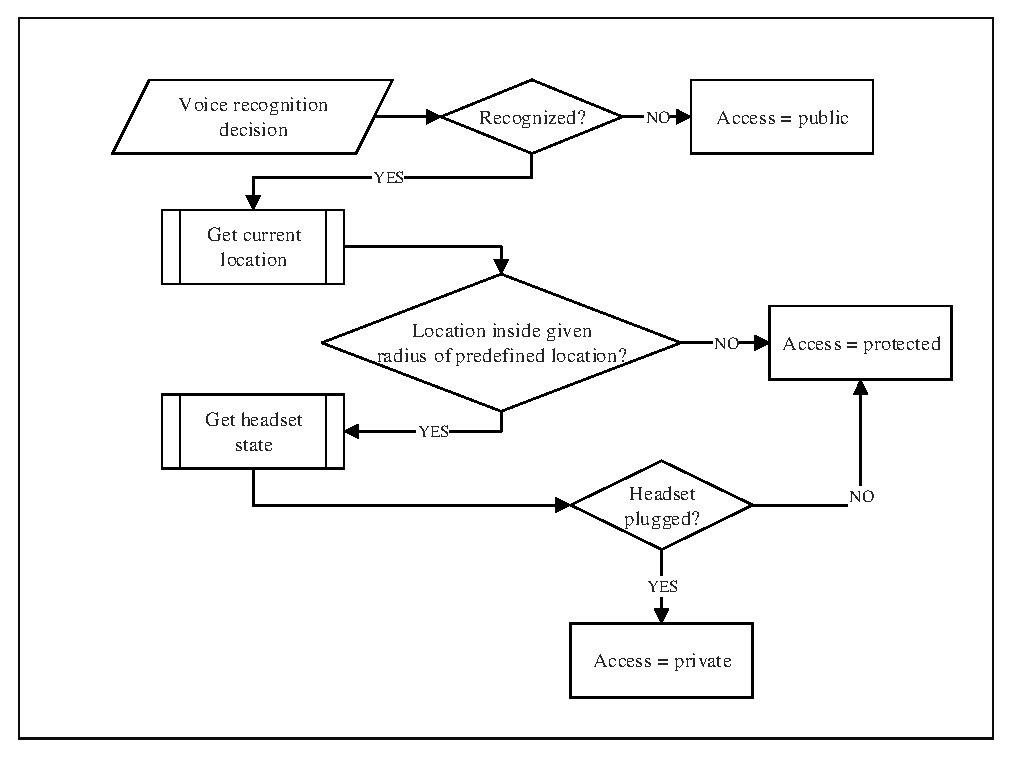
\includegraphics[width=10 cm]{6.eps}
	\caption{Flowchart of the decision-making process.}
	\label{fig:6}
\end{figure}

%%%%%%%%%%%%%%%%%%%%%%%%%%%%%%%%%%%%%%%%%%
\section{Experiments}

The experiment we have conducted aims at assessing the proposed authentication system. Moreover, it let us suggest a public data set of 11 speakers voice features (\textit{i.e.} UQAC-Studs). To achieve this, every participant used the system to authenticate himself or herself on the provided mobile device, with a headset plugged. Two distinct environmental conditions were exploited in this experiment. The first one was a quiet environment, where the training process and a quiet authentication were completed. Finally, another authentication attempt was performed within a noisy environment in order to evaluate the robustness of such a mechanism.

%%%%%%%%%%%%%%%%%%%%%%%%%%%%%%%%%%%%%%%%%%
\subsection{Participants}

We recruited 11 university students as participants, 7 males, and 4 females from 19 to 36 years. All participants were speaking French but some distinct accent, such as Canadian French and hexagonal French were observed. Moreover, they were either \textit{iOS}, or \textit{Android} users and owned at least one recent mobile device (\textit{i.e.} smartphone or tablet). Furthermore, 9 of the participants used an unlocking mechanism for their smartphone (PIN: 4, pattern: 2, fingerprint: 3) and fingerprint users either had a PIN code, or a pattern as fallback mechanism.

%%%%%%%%%%%%%%%%%%%%%%%%%%%%%%%%%%%%%%%%%%
\subsection{Data Collection}

The proposed text-independent system was implemented as an \textit{Android} application which requires at least the 4.0.1 version of the mobile operating system. Figure \ref{fig:7} shows screen captures of the application. All participants performed the experiment on the same smartphone (\textit{i.e.} \textit{LG Nexus 5} running \textit{Android} 6.0.1 with a \textit{Snapdragon 800} Quad-core at 2.3 GHz CPU and 2 GB of RAM) with the same headset (\textit{i.e.} \textit{Bose SoundTrue I}) in same conditions (\textit{i.e.} room and public place).

Since it was desired to have real-environment recording conditions, a quiet room was selected to achieve the training, as well as the quiet identification session. Conversely, the noisy session was performed in the cafeteria of the University. The sound level of each distinct place was measured thanks to a sound level meter embedded in the application. The mean value evaluated reached 16.5 dB in the quiet environment while 95 dB was observed in the noisy one.

\begin{figure}[H]
	\centering
	\includegraphics[width=8 cm]{7.png}
	\caption{Screen captures of the \textit{Android} application.}
	\label{fig:7}
\end{figure}

%%%%%%%%%%%%%%%%%%%%%%%%%%%%%%%%%%%%%%%%%%
\subsection{Procedure}

In the beginning, participants were introduced to the experimental procedure and the current position was added to the trusted location list.

Then, training participant voices was the first phase of the experiment. To complete such an operation, a text was randomly selected in a database and displayed on the screen of the device. Participants were instructed to wear the headset and to familiarize with the content. Once they were ready, participants were advised to start the recording by themselves and next, to begin reading the text aloud. The record was automatically stopped after one minute by the application and participants were warned through both a vibration and a text-to-speech synthesis system. At that point, participants were asked to wait until the end of the computation. In the meantime, the main recorded file was split into 10 seconds\textquoteright chunks, being 6 instances per class in total. Each set of features from each instance were written in the data set which was used to create the training model of the Na\"ive Bayes classifier, as described previously. Finally, participants were advised of the completion of the process thanks to a pop-up message.

At the end of the training process, the authentication process starts. This procedure was performed twice. In the first place, participants were asked to wear the headset and to pronounce the locution of their choice in the quiet environment. In the second place, they were requested to execute the same task in the noisy environment. Insofar as there was no restriction on the locution which had to be said\textemdash participants were able to use either two different expressions, or the same one for the two authentication sessions. Since every authentication attempts were performed in the same place, our decision-making has always stated that users stood in a trusted location. Therefore, we have mocked a location which was not considered as a trusted one afterwards, in order to verify the reliability of our technique. Figure \ref{fig:8} summarizes the proceedings of the experiment we conducted using a sequence diagram.

Finally, in the last step of the experiment, participants were sounded out about their habits concerning authentication on their own device, as well as their opinion as regards the proposed system.

\begin{figure}[H]
	\centering
	\includegraphics[width=10 cm]{8.png}
	\caption{Sequence diagram of the experiment.}
	\label{fig:8}
\end{figure}

%%%%%%%%%%%%%%%%%%%%%%%%%%%%%%%%%%%%%%%%%%
\section{Results and Discussion}

%%%%%%%%%%%%%%%%%%%%%%%%%%%%%%%%%%%%%%%%%%
\subsection{Speech Corpora}

In this research, we have evaluated the performance of our system by exploiting two additional speech corpora for comparison purpose with the data set we suggest.
The first one is the Ted-LIUM corpus which has been proposed by Rousseau \textit{et al.} \cite{33}. It includes a total of 1495 audio files extracted from TED talks, where all speeches are English-based with multiple distinct accents. These records are mono-channel, and they are encoded in 16-bit signed integer PCM at a 16 kHz sampling rate. Although the corpus was published using the NIST Sphere format (SPH), we required to convert the whole files in Waveform Audio File Format (WAV). Furthermore, we took care of removing the first fourth frames of each file, as they correspond to the talk opening sequence.
The second speech corpus that we have exploited in this research is a subset of the TIMIT corpus, which has been suggested by Garofolo \textit{et al.} \cite{34}. Such a subset contains 10 broadband recording files for 16 English-based speakers. Such provided files are also mono-channel and encoded in 16-bit integer PCM at a 16 kHz sampling rate.

%%%%%%%%%%%%%%%%%%%%%%%%%%%%%%%%%%%%%%%%%%
\subsection{Classification Performance Metrics}

Since classification let us predict at which registered speaker corresponds a given utterance; it is important to evaluate the performance of our system thanks to representative metrics. To this end, the accuracy is probably the most dominant measure in the literature, because of its simplicity. This measure provides the ratio between the correct number of predictions and the total number of cases given as,

\begin{equation}
\label{eq:15}
  	accuracy = \frac{TP+TN}{TP+TN+FP+FN}~,
\end{equation}

\noindent where $TP$ and $TN$ refer to true positive and true negative predictions respectively, and the total additionally include false positive ($FP$) and false negative ($FN$) predictions.

Despite its popularity, accuracy alone does typically not provide enough information to evaluate the robustness of prediction outcomes. Indeed, accuracy does not compensate for results that may be expected by luck. Indeed, a high accuracy does not necessarily reflect an indicator of a high classification performance. This is the accuracy paradox. For instance, in a predictive classification setting, predictive models with a given level of accuracy may have greater predictive power than models with higher accuracy. In that sense, as suggested by Ben-David \cite{35}, we decided to provide the Cohen\textquoteright s kappa evaluation metric as well. This measure takes into account such a paradox and remains a more relevant metric in multiclass classification evaluations such as our system. The kappa measure is given by,

\begin{equation}
\label{eq:16}
  	kappa = \frac{P_o-P_e}{1-P_e}~,
\end{equation}

\noindent where $P_o$ and $P_e$ are the observed and the expected probabilities respectively.

%%%%%%%%%%%%%%%%%%%%%%%%%%%%%%%%%%%%%%%%%%
\subsection{Results Obtained}

The performance of our proposed system was evaluated according to several analyses. First of all, results of the experiment we described previously are shown in Table \ref{tab:2}. In this evaluation, we have exploited testing instances we obtained over our experiment for both quiet and noisy environments. Thanks to such achieved results it is possible to observe that our system yields an acceptable identification of voices in real environmental conditions with our instances.

\begin{table}[H]
\caption{Results of the experiment based on the realized data set: UQAC-Studs.}
\centering
\label{tab:2}
	\begin{tabular}{rcc}
		\noalign{\smallskip}\hline\noalign{\smallskip}
		& \textbf{Quiet environment} & \textbf{Noisy environment}\\
		\noalign{\smallskip}\hline\noalign{\smallskip}
		Accuracy & 91\% & 82\%\\		
		Kappa & 90\% & 80\%\\
		Total classes & 11 & 11\\
		Total instances for training & 5 & 5\\
		Total instances for identification & 1 & 1\\
		\noalign{\smallskip}\hline
	\end{tabular}
\end{table}

However, since it is impossible to state the reliability of the results we obtained with only such data, we have constructed related data sets thanks to the Ted-LIUM and the TIMIT subset corpora as a means of comparison for our system. 
For all 16 speakers, the TIMIT subset admits ten recorded files between two and four seconds. Hence, we have exploited 6 samples to construct the training set and the four remaining were used for the identification. Results we obtained over this speech corpus are shown in Table \ref{tab:3}.

\begin{table}[H]
\caption{Results obtained over a subset of the TIMIT speech corpus.}
\centering
\label{tab:3}
\begin{tabular}{rc}
	\hline\noalign{\smallskip}
		Accuracy & 83\% \\
		Kappa & 82\% \\
		Total classes & 16\\
		Total instances for training & 6\\
		Total instances for identification & 4\\
	\noalign{\smallskip}\hline
\end{tabular}
\end{table}

Nevertheless, since the Ted-LIUM speech corpus is large and contains several long records, we judged that it was a necessity to unify the construction of the data sets according to the previously described subset of TIMIT corpus. In that sense, we have created ten different training sets by selecting 16 samples randomly over the 1495 files. Moreover, we have also ensured that a sample was not chosen more than once for a given batch. For each batch of ten records, every sample is split into 10 instances of 5 seconds. In order to be more consistent with our experimental procedure, the first 6 instances are used in the training phase; while the last four are exploited for the identification. Figure \ref{fig:9} details the results obtained for these ten random batches. In addition, such an experiment has revealed a mean accuracy of 87\% and a mean kappa measure of 85\%. 

\begin{figure}[H]
	\centering
	\includegraphics[width=10 cm]{9.png}
	\caption{Accuracy and kappa measures achieved by our system over the 10 random batches of the Ted-LIUM corpus we have created.}
	\label{fig:9}
\end{figure}

However, as these evaluations involve a relatively small number of distinct classes, we point out the analysis of the evolution of the kappa measure when increasing the number of classes. The Ted-LIUM corpus let us perform such an appraisal since it is the largest corpus we used in this research. Hence, we did not change the number of instances that we have exploited in the previous evaluation, six instances per class for the training and four for the identification phase. We chose to compute the kappa by increasing the number of classes exponentially until reaching the closest value to the total of 1495 records. Figure \ref{fig:10} shows that the more there are classes, the more the kappa measure tends to decrease. Indeed, our system obtains a kappa of 47\% where the entire set of classes was used in the identification process. Such a result was expected since we are not facing a binary classification problem.

\begin{figure}[H]
	\centering
	\includegraphics[width=10 cm]{10.png}
	\caption{Evolution of the kappa measure over the Ted-LIUM corpus when increasing the number of classes exponentially.}
	\label{fig:10}
\end{figure}

Finally, an empirical comparison between our proposed method and previous works is exposed in Table \ref{tab:4}.

\begin{table}[H]
\centering
\caption{Empirical comparison between our text-independent speaker authentication and previous works.}
\label{tab:4}
\resizebox{1\columnwidth}{!} 
{
	$\begin{tabular}{rccccc}
		\noalign{\smallskip}\hline\noalign{\smallskip}
		& \textbf{Features} & \textbf{\#Features} & \makecell{\textbf{Classification, } \\ \textbf{Pattern Matching}} & \textbf{Accuracy} & \textbf{Dataset}\\
		\noalign{\smallskip}\hline\noalign{\smallskip}\noalign{\smallskip}

		\textbf{Thullier\textit{ et al.}} & LPCCs & 20 & Na\"ive Bayes & \makecell{91\%$\sim$82\% \\ 87\% \textit{(avg)} \\ 83\%} & \makecell{UQAC-Studs \\ Ted-LIUM \\ TIMIT (subset)}\\

		\noalign{\smallskip}		
		
		\textbf{Nair and Salam \cite{19}} & LPCs \& LPCCs & \makecell{20, 30 \\ \& 40} & DTW & \makecell{90.4\% \textit{(20 LPCs)} \\ 94.8\% \textit{(20 LPCCs)}} & TIMIT\\
		
		\noalign{\smallskip}
		
		\textbf{Reynolds and Rose \cite{20}} & MFCCs & \makecell{100 12-dimensional \\ vectors per second}  & GMM & \makecell{96.8\% \\ 80.8\%} & \makecell{KING \\ Private samples}\\
		
		\noalign{\smallskip}
		
		\textbf{Kumar \textit{et al.} \cite{18}} & \makecell{LPCs, LPCCs, \\ RC, LAR, \\ ARCSIN \& LSF } & N.A. & \makecell{ANN \\ \textit{(backpropagation)}} & 85.74\% & Private samples\\
		
		\noalign{\smallskip}\hline
		
	\end{tabular}$
}
\end{table}

%%%%%%%%%%%%%%%%%%%%%%%%%%%%%%%%%%%%%%%%%%
\subsection{Replay Attacks}

Replay attacks refer to the presentation of a recorded audio sample of a genuine voice played-back to get access to the protected system \cite{41}. Since this kind of attack is considered to be the major security drawback of voice-based authentication mechanisms, it is relevant for us to state about the robustness of our system as it stands. Indeed, no specific method to counteract replay attacks such as \cite{42} has been implemented in this work.

In order to proceed such an evaluation, the testing instance, for each participant of our experiment, was replayed to the authentication system through a standard desktop computer speaker. As expected, six utterances over the eleven were genuinely identified without the headset. However none fraudulent samples were correctly identified while using the headset which embeds its own microphone.

%%%%%%%%%%%%%%%%%%%%%%%%%%%%%%%%%%%%%%%%%%
\subsection{Computation Performances Considerations}

Since we desired to create a user-centered text-independent speaker authentication mechanism, we judge that an efficient, as well as a reliable implementation is an important angle when considering to replace most used and weak authentication mechanisms such as PIN codes. 

To this end, we have chosen suitable techniques with attention to time complexity and memory consumption. Figure \ref{fig:11} exposes a profiling of CPU, memory and battery utilization of the mobile device, in relation to the cumulative time consumption. These measurements were performed on every stage of the training, as well as the identification processes, for one given instance of the data set we suggest. Moreover, the start stage was considered as an idle state for the application.

In order to produce six instances of ten seconds each, we had to record during 60 seconds. Hence, the whole training process has required less than ten seconds of processing, while the identification process has demanded less than 500 ms to terminate since we recorded during two seconds. Moreover, the memory usage did not exceed 70 MB.

These measurements were observed through the \textit{Trepn Profiler} application developed by \textit{Qualcomm}, but since accurate performance metrics are difficult to obtain, it is impossible for us to provide a suitable analysis of the battery needs. Nevertheless, we only present a trend of the required power consumption for the application.

\begin{figure}[H]
	\centering
	\includegraphics[width=10 cm]{11.png}
	\caption{CPU, RAM, battery and time consumption, respectively expressed in \%CPU, MB, mW and seconds, over every stage of the experiment, where the first chart refers to the training process and the second is the identification.}
	\label{fig:11}
\end{figure}

%%%%%%%%%%%%%%%%%%%%%%%%%%%%%%%%%%%%%%%%%%
\subsection{Participants Opinion Considerations}

Here we report participants\textquoteright opinions concerning the proposed system. Hence, it aims at better understanding users\textquoteright needs and habits as regards authentication in order to replace present mechanisms offered on mobile devices. This survey showed that two of the five users who have enabled a knowledge-based authentication mechanism (\textit{i.e.} PIN or pattern) have reported that it is overly repetitive and lead them to make mistakes several times a day. Besides, all three fingerprints users have mentioned a disturbing dysfunction with finger moisture. As a result, three participants over the nine who locked their device, as well as one over the two participants who did not employ such security, would use this system as a replacement of their present authentication scheme because of its simplicity. Moreover, eight respondents have mentioned they could place their confidence in the described system. However, the three remaining participants have declared that talking to their mobile device could be annoying in public areas and consequently, they have claimed that they do not trust any voice-based authentication scheme. Nevertheless, these three participants have conceded that a continuous authentication without even mind about it, was seductive and they all declared that they would be less worried to use, daily, a system that does not transmit data over the network (even if they are encrypted).

%%%%%%%%%%%%%%%%%%%%%%%%%%%%%%%%%%%%%%%%%%
\subsection{Discussion}

Firstly, based on the results we have obtained in previous sections, it is possible for us to observe that the rate of correct identification remains consistent when our data set is compared to the ones we have built through both the Ted-LIUM and a subset of the TIMIT corpora. Moreover, these results stand relatively similar to the ones obtained by Kumar \textit{et al.} \cite{18} but not as good as the ones achieved by Nair and Salam \cite{19} as exposed in Table \ref{tab:4}. Nevertheless, since we  have also exploited LPCCs as discriminating voice features, it is possible for us to say that our classification algorithm remains theoretically less expensive than a DTW-based solution that involves quadratic time and space complexities. Due to the use of LPCCs features, comparing our technique directly with MFCCs-based ones is very limited. However, according to the comparative detailed in Table \ref{tab:4} the results achieved by our proposed system also remain consistent in regard to the work of Reynolds and Rose \cite{20}. Moreover, the reliability of our proposed system stand acceptable, in real life recording conditions, with a small number of classes; that is, the common use case of authentication mechanisms (\textit{i.e.} the mobile device owner and potentially one or two more people). The results obtained with fraudulent utterances of speakers that participate to our experiment lead us to state that our system is perfectible in terms of fraudulent access though replayed audio samples. However the decision-making process suggested in this work should significantly reduce risks involved. Indeed, since none of the played-back samples misled the authentication mechanisms when the headset is involved, attackers will only have access to the content with a \textit{protected} access that refers to non-critical piece of information mobile devices may contain. Hence, by introducing the notion of access privileges, we also aim at reducing unsafe situations in case of false acceptance identifications.

Secondly, the participants\textquoteright opinion collection allows us to state that our system could be a relevant authentication mechanism for several users. In addition, since it is text-independent, such a system, with a few modifications, could perform the authentication in a continuous manner, without any involvement from the user. In that sense, anxieties, as regards the discomfort in talking to a device in public places, which were reported in the past may be reduced to void. Therefore, we esteem that such a technique may be a more significant option as part of a multilayer authentication. Moreover, it should also be better employed as a more reliable fallback solution in order to eradicate PIN codes.

%%%%%%%%%%%%%%%%%%%%%%%%%%%%%%%%%%%%%%%%%%
\section{Conclusions}

In this research, we have proposed the design of a text-independent speaker authentication system for mobile devices with a specific focus on its usability. This implementation operates as stand-alone which does not require any network communications. Indeed, both training and identification phases, which are based on LPCCs and the Na\"ive Bayes classifier, are achieved onto the device itself. Moreover, we have enhanced the identification thanks to a decision-making that substantially relies on user locations and the presence of a headset. Results we have obtained over the different analysis we have performed, suggest that it embodies a reliable and efficient authentication mechanism in both quiet and noisy environments (\textit{i.e.} 90\% and 80\% of kappa in quiet and noisy environments, respectively), capable of running on weakest mobile devices. 

We found that 7 users were still not ready to switch from their present authentication mechanism. Moreover, three of the participants have reported that they could not place their confidence in such a system, as it may be disturbing when used in public places. However, since it is text-independent, legitimate users may be implicitly authenticated as they start speaking, insofar as the mobile device is neither in their pocket, nor their bag (\textit{i.e.} during a conversation). In that sense, since the idea of being authenticated in a continuous manner was seducing to skeptical  participants, we also suggest that this technique should be either used in a multilayer authentication system, or as a fallback mechanism, namely when the first one fails, to cover most of the users\textquoteright needs and usages.

%%%%%%%%%%%%%%%%%%%%%%%%%%%%%%%%%%%%%%%%%%
\section{Future works}

Future works will focus on offering the application on the \textit{Google Play Store} to better assess the accuracy and the robustness of the proposed authentication system. However, the current implementation will be adapted in order to let us track user authentication attempt outcomes and locations. In this way, such a large-scale evaluation will provide more reliable results in front of real life condition usages and the location-based decision will be better exploited and significant, as it was in the experiment we have conducted in this research. Besides, the extraction of MFCCs discriminating voice features will be considered in order to produce a direct comparison in terms of reliability and effectiveness with LPCCs features.

%%%%%%%%%%%%%%%%%%%%%%%%%%%%%%%%%%%%%%%%%%

\vspace{6pt} 

%%%%%%%%%%%%%%%%%%%%%%%%%%%%%%%%%%%%%%%%%%
\acknowledgments{Authors would like to acknowledge S\'ebastien Gaboury and Val\`ere Plantevin for their conscientious reviews, as well as every person who participates in our experiment.}

%%%%%%%%%%%%%%%%%%%%%%%%%%%%%%%%%%%%%%%%%%
\authorcontributions{The authors contributed in equal parts.}

%%%%%%%%%%%%%%%%%%%%%%%%%%%%%%%%%%%%%%%%%%
\conflictsofinterest{The authors declare no conflict of interest.} 

%%%%%%%%%%%%%%%%%%%%%%%%%%%%%%%%%%%%%%%%%%
%% optional
\abbreviations{The following abbreviations are used in this manuscript:\\

\noindent 
\begin{tabular}{@{}ll}
ANN & Artificial Neural Network\\
CDBN & Convolutional Deep Belief Networks\\
DBFS & Decibels Relative to Full Scale\\
DTW & Dynamic Time Warping\\
EER & Equal Rerror Rate\\
GMM & Gaussian Mixture Model\\
HMM & Hidden Markov Model\\
LPC & Linear Prediction Coefficient\\
LPCC & Linear Prediction Cepstral Coefficient\\
MFCC & Mel-Frequency Cepstral Coefficient\\
PCM & Pulse-Code Modulation\\
PIN & Personal Identification Number\\
SPH & NIST Sphere Format\\
VAD & Voice Activity Detection\\
VQ & Vector Quantization\\
WAV & Waveform Audio File Format
\end{tabular}}

%=====================================
% References, variant B: external bibliography
%=====================================
\externalbibliography{yes}
\bibliography{refs} 

%%%%%%%%%%%%%%%%%%%%%%%%%%%%%%%%%%%%%%%%%%
\end{document}

